\documentclass{article}
\usepackage{tikz}
\usetikzlibrary{automata,arrows}
\setlength\parindent{24pt}
\begin{document}
Example0
\\
$ M_{L_3}^{G_1}$ :
\\
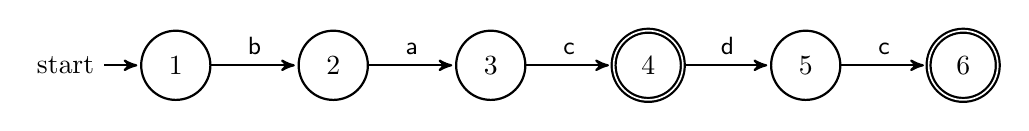
\begin{tikzpicture}[->,>=stealth',shorten >=1pt,auto,node distance=2cm,
    thick,main node/.style={circle,draw,font=\sffamily\Large\bfseries}]

\node[initial, state] (1) {1};
\node[state] (2) [right of=1] {2};
\node[state] (3) [right of=2] {3};
\node[state, accepting] (4) [right of=3] {4};
\node[state] (5) [right of=4] {5};
\node[state, accepting] (6) [right of=5] {6};

\path[every node/.style={font=\sffamily\small}]
(1) edge node {b} (2)
(2) edge node {a} (3)
(3) edge node {c} (4)
(4) edge node {d} (5)
(5) edge node {c} (6)
;

\end{tikzpicture}
\\
% $ M_{L_4}^{G_1}$ :
% \\
% \begin{tikzpicture}[->,>=stealth',shorten >=1pt,auto,node distance=2cm,
%     thick,main node/.style={circle,draw,font=\sffamily\Large\bfseries}]

% \node[initial, state] (1) {1};
% \node[state] (2) [right of=1] {2};
% \node[state] (3) [right of=2] {3};
% \node[state] (4) [right of=3] {4};
% \node[state, accepting] (5) [right of=4] {5};
% \node[state, accepting] (6) [below of=2] {6};

% \path[every node/.style={font=\sffamily\small}]
% (1) edge node {b} (2)
% (2) edge node {a} (3)
% (3) edge node {c} (4)
% (4) edge node {d} (5)
% (2) edge node {c} (6)
% ;

% \end{tikzpicture}
% \\
$ M_{L_3}^{G_3}$ :
\\
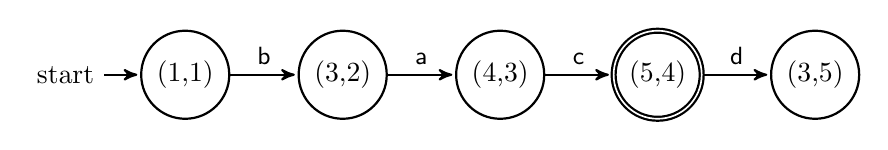
\begin{tikzpicture}[->,>=stealth',shorten >=1pt,auto,node distance=2cm,
    thick,main node/.style={circle,draw,font=\sffamily\Large\bfseries}]

\node[initial, state] (1) {(1,1)};
\node[state] (2) [right of=1] {(3,2)};
\node[state] (3) [right of=2] {(4,3)};
\node[state, accepting] (4) [right of=3] {(5,4)};
\node[state] (5) [right of=4] {(3,5)};


\path[every node/.style={font=\sffamily\small}]
(1) edge node {b} (2)
(2) edge node {a} (3)
(3) edge node {c} (4)
(4) edge node {d} (5)
;

\end{tikzpicture}

$ M_{L_3}^{G_4}$ : \\
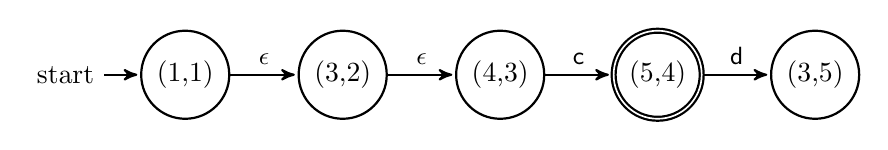
\begin{tikzpicture}[->,>=stealth',shorten >=1pt,auto,node distance=2cm,
    thick,main node/.style={circle,draw,font=\sffamily\Large\bfseries}]

\node[initial, state] (1) {(1,1)};
\node[state] (2) [right of=1] {(3,2)};
\node[state] (3) [right of=2] {(4,3)};
\node[state, accepting] (4) [right of=3] {(5,4)};
\node[state] (5) [right of=4] {(3,5)};


\path[every node/.style={font=\sffamily\small}]
(1) edge node {$\epsilon$} (2)
(2) edge node {$\epsilon$} (3)
(3) edge node {c} (4)
(4) edge node {d} (5)
;

\end{tikzpicture}


$ M_{L_3}^{G_5}$ : \\
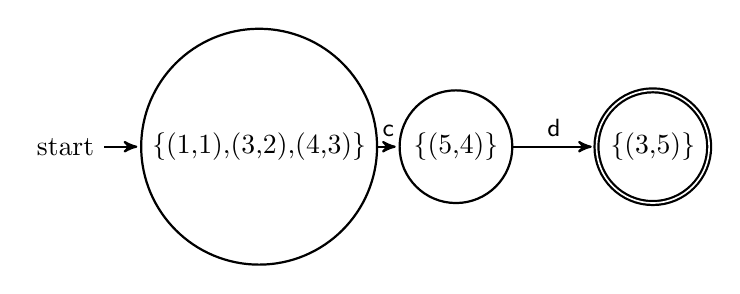
\begin{tikzpicture}[->,>=stealth',shorten >=1pt,auto,node distance=2.5cm,
    thick,main node/.style={circle,draw,font=\sffamily\Large\bfseries}]

\node[initial, state] (1) {\textrm{\{(1,1), \\ (3,2), \\ (4,3)\}}};
\node[state] (2) [right of=1] {\{(5,4)\}};
\node[state, accepting] (3) [right of=2] {\{(3,5)\}};



\path[every node/.style={font=\sffamily\small}]
(1) edge node {c} (2)
(2) edge node {d} (3)
;

\end{tikzpicture}

$ M_{L_4}^{G_1}$ :
\\
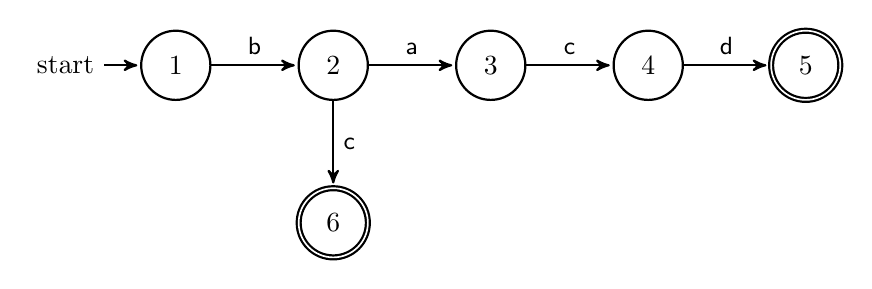
\begin{tikzpicture}[->,>=stealth',shorten >=1pt,auto,node distance=2cm,
    thick,main node/.style={circle,draw,font=\sffamily\Large\bfseries}]

\node[initial, state] (1) {1};
\node[state] (2) [right of=1] {2};
\node[state] (3) [right of=2] {3};
\node[state] (4) [right of=3] {4};
\node[state, accepting] (5) [right of=4] {5};
\node[state, accepting] (6) [below of=2] {6};

\path[every node/.style={font=\sffamily\small}]
(1) edge node {b} (2)
(2) edge node {a} (3)
(3) edge node {c} (4)
(4) edge node {d} (5)
(2) edge node {c} (6)
;

\end{tikzpicture}

$ M_{L_4}^{G_3}$ :
\\
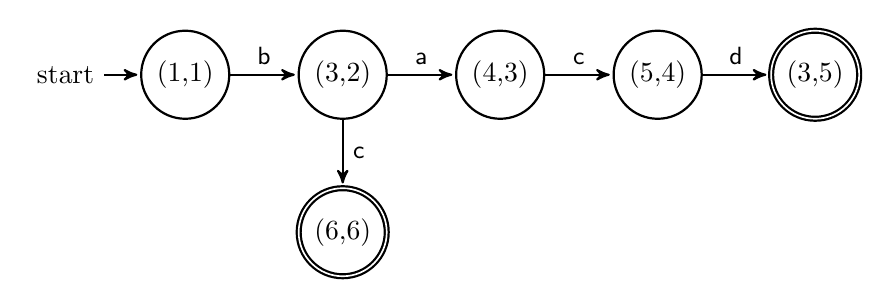
\begin{tikzpicture}[->,>=stealth',shorten >=1pt,auto,node distance=2cm,
    thick,main node/.style={circle,draw,font=\sffamily\Large\bfseries}]

\node[initial, state] (1) {(1,1)};
\node[state] (2) [right of=1] {(3,2)};
\node[state] (3) [right of=2] {(4,3)};
\node[state] (4) [right of=3] {(5,4)};
\node[state, accepting] (5) [right of=4] {(3,5)};
\node[state, accepting] (6) [below of=2] {(6,6)};

\path[every node/.style={font=\sffamily\small}]
(1) edge node {b} (2)
(2) edge node {a} (3)
(3) edge node {c} (4)
(4) edge node {d} (5)
(2) edge node {c} (6)
;

\end{tikzpicture}

$ M_{L_4}^{G_4}$ : \\
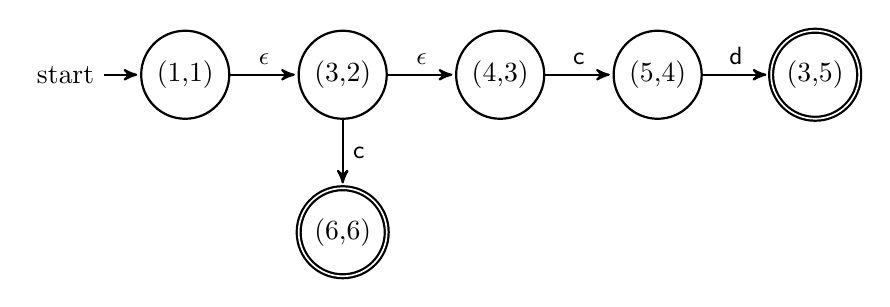
\begin{tikzpicture}[->,>=stealth',shorten >=1pt,auto,node distance=2cm,
    thick,main node/.style={circle,draw,font=\sffamily\Large\bfseries}]
\node[initial, state] (1) {(1,1)};
\node[state] (2) [right of=1] {(3,2)};
\node[state] (3) [right of=2] {(4,3)};
\node[state] (4) [right of=3] {(5,4)};
\node[state, accepting] (5) [right of=4] {(3,5)};
\node[state, accepting] (6) [below of=2] {(6,6)};

\path[every node/.style={font=\sffamily\small}]
(1) edge node {$\epsilon$} (2)
(2) edge node {$\epsilon$} (3)
(3) edge node {c} (4)
(4) edge node {d} (5)
(2) edge node {c} (6)
;

\end{tikzpicture}


$ M_{L_4}^{G_5}$ : \\
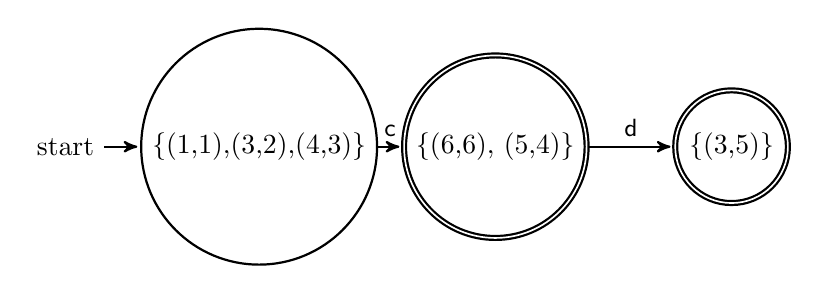
\begin{tikzpicture}[->,>=stealth',shorten >=1pt,auto,node distance=3cm,
    thick,main node/.style={circle,draw,font=\sffamily\Large\bfseries}]

\node[initial, state] (1) {\textrm{\{(1,1), \\ (3,2), \\ (4,3)\}}};
\node[state, accepting] (2) [right of=1] {\{(6,6), (5,4)\}};
\node[state, accepting] (3) [right of=2] {\{(3,5)\}};



\path[every node/.style={font=\sffamily\small}]
(1) edge node {c} (2)
(2) edge node {d} (3)
;

\end{tikzpicture}


\end{document}
    